\documentclass[12pt, titlepage]{article}

\usepackage{float}
\usepackage{geometry}
\usepackage{booktabs}
\usepackage{tabularx}
\usepackage{hyperref}
\usepackage{siunitx}
\hypersetup{
    colorlinks,
    citecolor=blue,
    filecolor=black,
    linkcolor=red,
    urlcolor=blue
}
\usepackage[round]{natbib}
\usepackage{amsmath, mathtools}
\usepackage{xr}
\externaldocument{../SRS/SRS}

\input{../Comments}
%% Common Parts

\newcommand{\progname}{Baja Dynamics} % PUT YOUR PROGRAM NAME HERE
\newcommand{\authname}{Team \#17, Team Name
\\ Grace McKenna
\\ Travis Wing
\\ Cameron Dunn
\\ Kai Arseneau} % AUTHOR NAMES                  

\usepackage{hyperref}
    \hypersetup{colorlinks=true, linkcolor=blue, citecolor=blue, filecolor=blue,
                urlcolor=blue, unicode=false}
    \urlstyle{same}
                                



\begin{document}

\title{System Verification and Validation Plan for \progname{}} 
\author{\authname}
\date{\today}
	
\maketitle

\pagenumbering{roman}

\section*{Revision History}

\begin{tabularx}{\textwidth}{p{3cm}p{2cm}X}
\toprule {\bf Date} & {\bf Version} & {\bf Notes}\\
\midrule
October 11th, 2024 & 0 & First version of VnV extra report\\
April 1st, 2025 & 1 & Added real-world data into VnV extra\\
\bottomrule
\end{tabularx}

~\\

\newpage

\tableofcontents

\listoftables


\listoffigures


\newpage

\section{Symbols, Abbreviations, and Acronyms}

\begin{table}[h]
  \raggedright
  \begin{tabular}{l l} 
    \toprule		
    \textbf{acronym} & \textbf{definition}\\
    \midrule
    CVT & Continuous Variable Transmission\\
    GPS & Global Positioning System\\
    IMU & Inertial Measurement Unit\\
    VnV & Verification and Validation\\
    \bottomrule
  \end{tabular}
  \caption{Verification and Validation Acronyms}
  \label{tab:vnv_acronyms}
\end{table}

\newpage

\pagenumbering{arabic}

\section{General Information}

\subsection{Summary}

\noindent This document will go into detail on the real-world data validation performed for the \progname{}. As per Dr. Smith's instructions, it will be completed prior to the course's end. This document currently serves as a placeholder for the final VnV extra report.

\section{Functional Tests Evaluation}

\subsection{Simulation Model}

\subsubsection{Position}

\begin{figure}[H]
  \begin{center}
   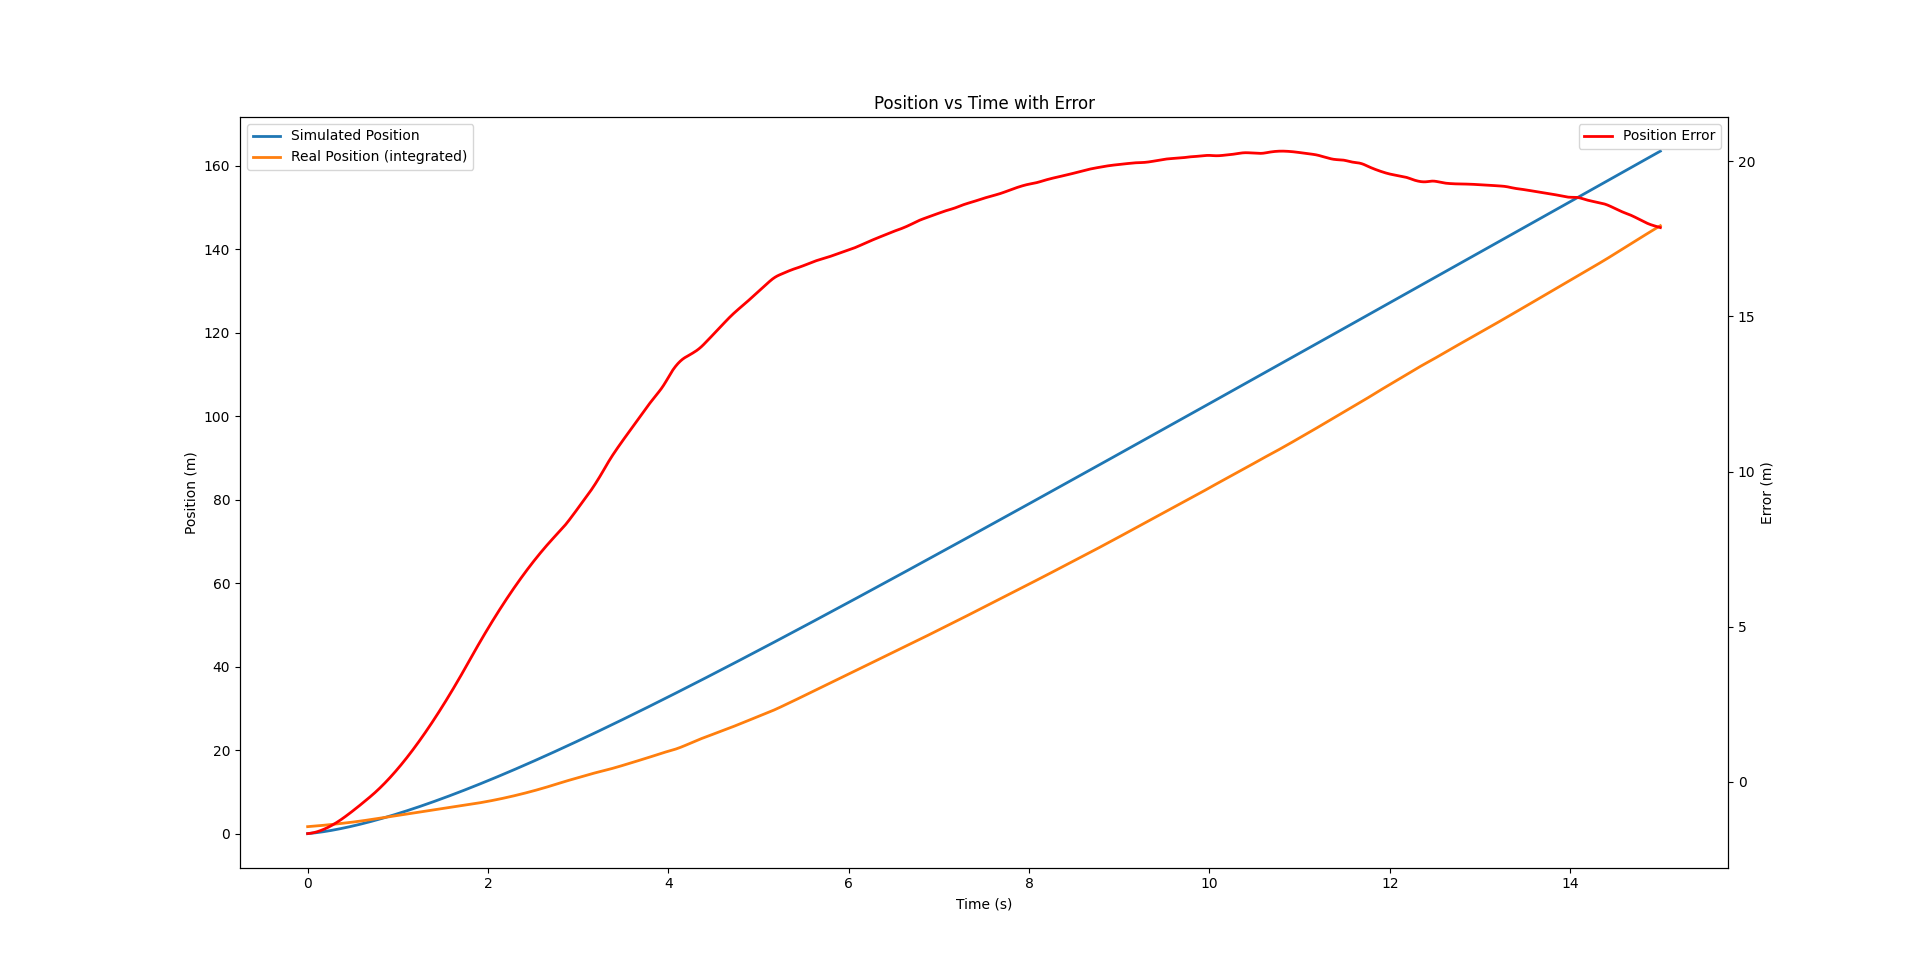
\includegraphics[width=\textwidth]{MSE Graphs/position.png}
  \caption{MSE of simulated position vs integrated experimental data.}
  \label{Fig_Position} 
  \end{center}
\end{figure}

\textbf{Overview of the Position vs. Time Plot:}  

The figure compares three key quantities over time:
\begin{itemize}
    \item Simulated Position (blue line)
    \item Measured (Integrated) Real Position (orange line)
    \item Position Error (red line), which is displayed on a secondary vertical axis.
\end{itemize}

\textbf{Initial Observation - Simulated Speed is Too High:}
Early in the plot, the simulated position exceeds the real position, indicating that the simulation predicts a higher velocity than observed. This discrepancy likely arises from an incomplete representation of resistive forces such as air resistance, rolling resistance, and friction.

\textbf{Mid to Late Observation - Error Dynamics:}  
Towards the end of the test, the error (red line) decreases slightly. This may be due to the model overestimating the final air resistance while underestimating other forces, such as friction and rolling resistance, which results in a final simulated speed that is still somewhat higher than reality, but still shows the initial descrepency.

\textbf{Testing Limitations - No Maximum Velocity Achieved:}  
The testing environment does not allow the car to reach its true maximum velocity. Consequently, the model cannot be fully validated at higher speeds, and any inaccuracies in modeling high-speed resistive forces remain untested.

\textbf{Conclusions:}
\begin{itemize}
    \item \textbf{Main Issue:} The simulation overestimates vehicle speed due to an oversimplified treatment of resistive forces.
    \item \textbf{Error Trends:} The narrowing gap between simulated and real positions toward the end suggests an overcompensation in the final air resistance term.
    \item \textbf{Future Work:} More comprehensive testing at higher speeds and enhanced modeling of resistive components (air drag, rolling friction, etc.) are needed to improve simulation fidelity.
\end{itemize}

\subsubsection{Velocity}

\begin{figure}[H]
  \begin{center}
   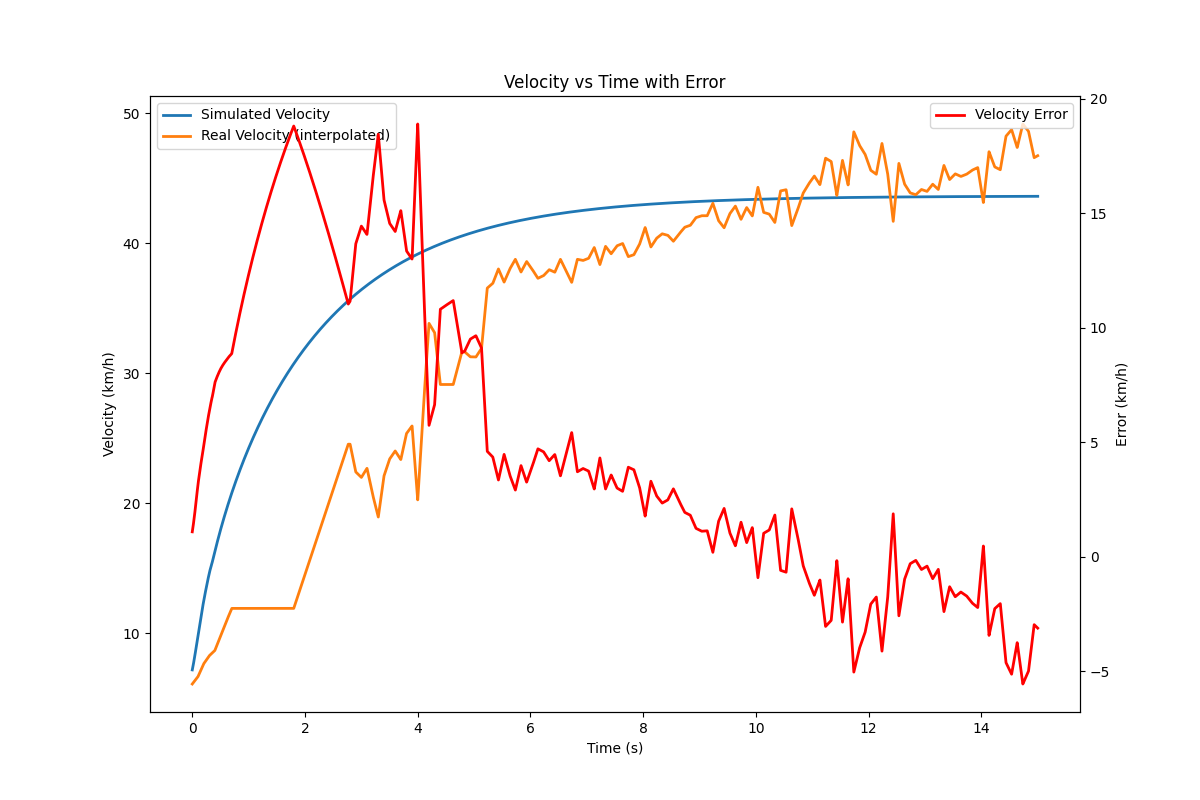
\includegraphics[width=\textwidth]{MSE Graphs/speed.png}
  \caption{MSE of simulated vehicle velocity and experimental data.}
  \label{Fig_Velocity} 
  \end{center}
\end{figure}

\textbf{Overview:}\\
The figure compares the simulated velocity (blue line) against the real, interpolated velocity (orange line), with the velocity error (red line) shown on a secondary vertical axis. Early in the plot, the simulated velocity is noticeably higher, indicating that certain resistive effects and potential slip conditions are not fully captured by the model. As time progresses, the two velocities begin to converge, although a measurable offset remains.

\textbf{Early Overestimation:}\\
During the initial phase, the simulation overestimates acceleration because it neglects several resistive forces (e.g., air resistance, rolling friction) and assumes no slipping. Without realistic slip modeling, the simulation applies full power to the wheels without the belt slippage that occur in real conditions.

\textbf{Later Convergence:}\\
As time goes on, the discrepancy between simulated and real velocities narrows, suggesting that the model's inaccuracies in resistive forces become less dominant at higher speeds. Nevertheless, an observable gap persists, implying that additional refinement of the resistance and slip models is necessary to achieve better accuracy.

\textbf{Comparison to Position Analysis:}\\
Many observations from the position error analysis also apply here. In both cases, the underlying cause is an oversimplified treatment of resistive forces and the lack of a slipping mechanism. Enhancing these aspects in the model would likely improve both position and velocity predictions.

\textbf{Conclusions:}
\begin{itemize}
    \item The simulation initially predicts excessive velocity due to ignoring key resistive forces and assuming perfect traction.
    \item Over time, simulated and real velocities partially align, though a consistent offset remains.
    \item More precise modeling of friction, rolling resistance, and slip is required for higher-fidelity velocity predictions.
\end{itemize}

\subsubsection{Acceleration}

\textbf{Acceleration Analysis:}\\
The plan includes a detailed investigation of the car's acceleration profile to further validate the simulation. Unfortunately, acceleration data has not yet been gathered, so a direct comparison with the model is not currently possible. Based on the trends observed in both the position and velocity analyses, we expect the following:

\begin{itemize}
    \item \textbf{Early Stage:} The simulation likely overestimates acceleration at the beginning, due to the simplified treatment of resistive forces (e.g., air resistance, friction) and the assumption of perfect traction.
    \item \textbf{Later Stage:} As time progresses, it is anticipated that the simulated acceleration will be lower than the actual values, mirroring the gradual convergence observed in the other parameters.
\end{itemize}

These expected trends suggest that, similar to the position and velocity results, the initial overestimation in acceleration will diminish over time, leading to a closer, yet still offset, match with the real-world data once it becomes available.

\subsubsection{Shift}

\begin{figure}[H]
  \begin{center}
   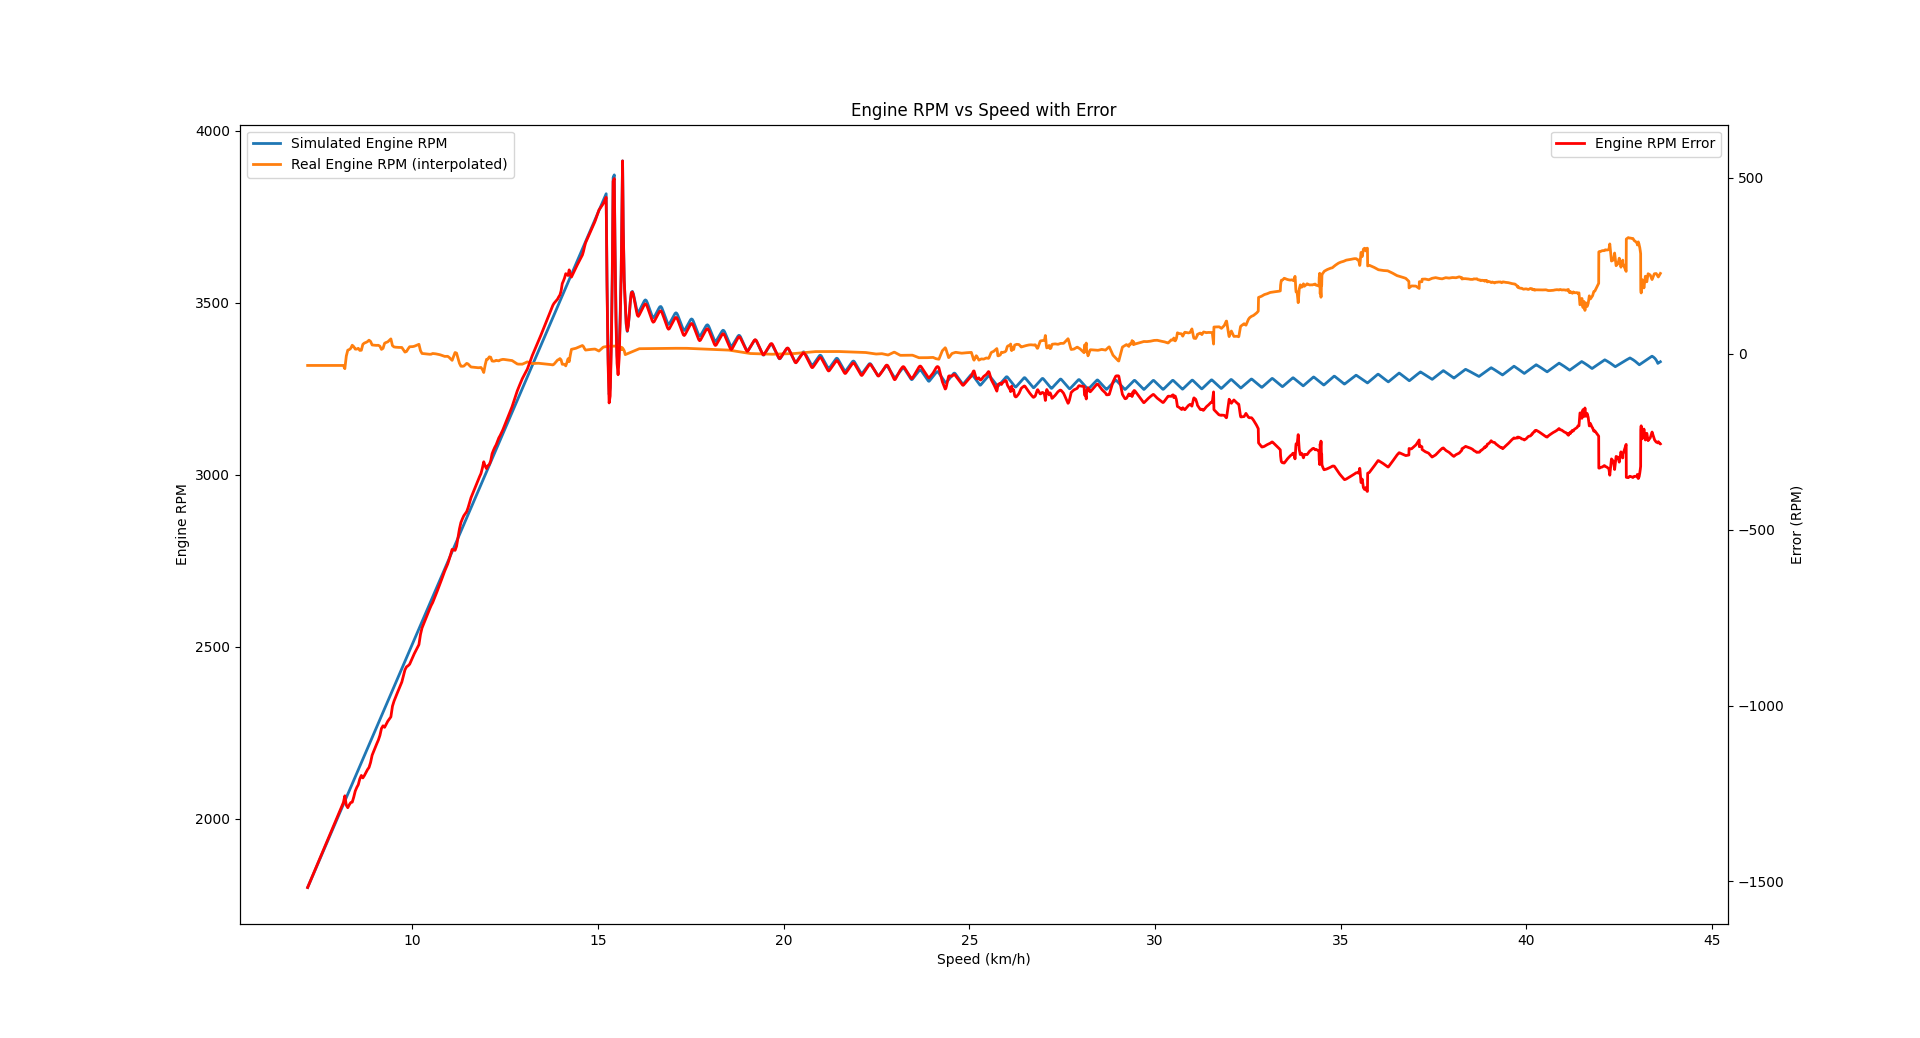
\includegraphics[width=\textwidth]{MSE Graphs/shift_curve_3400rpm.png}
  \caption{MSE of simulated shift curve and experimental data.}
  \label{Fig_Shift_3400} 
  \end{center}
\end{figure}

\begin{figure}[H]
  \begin{center}
   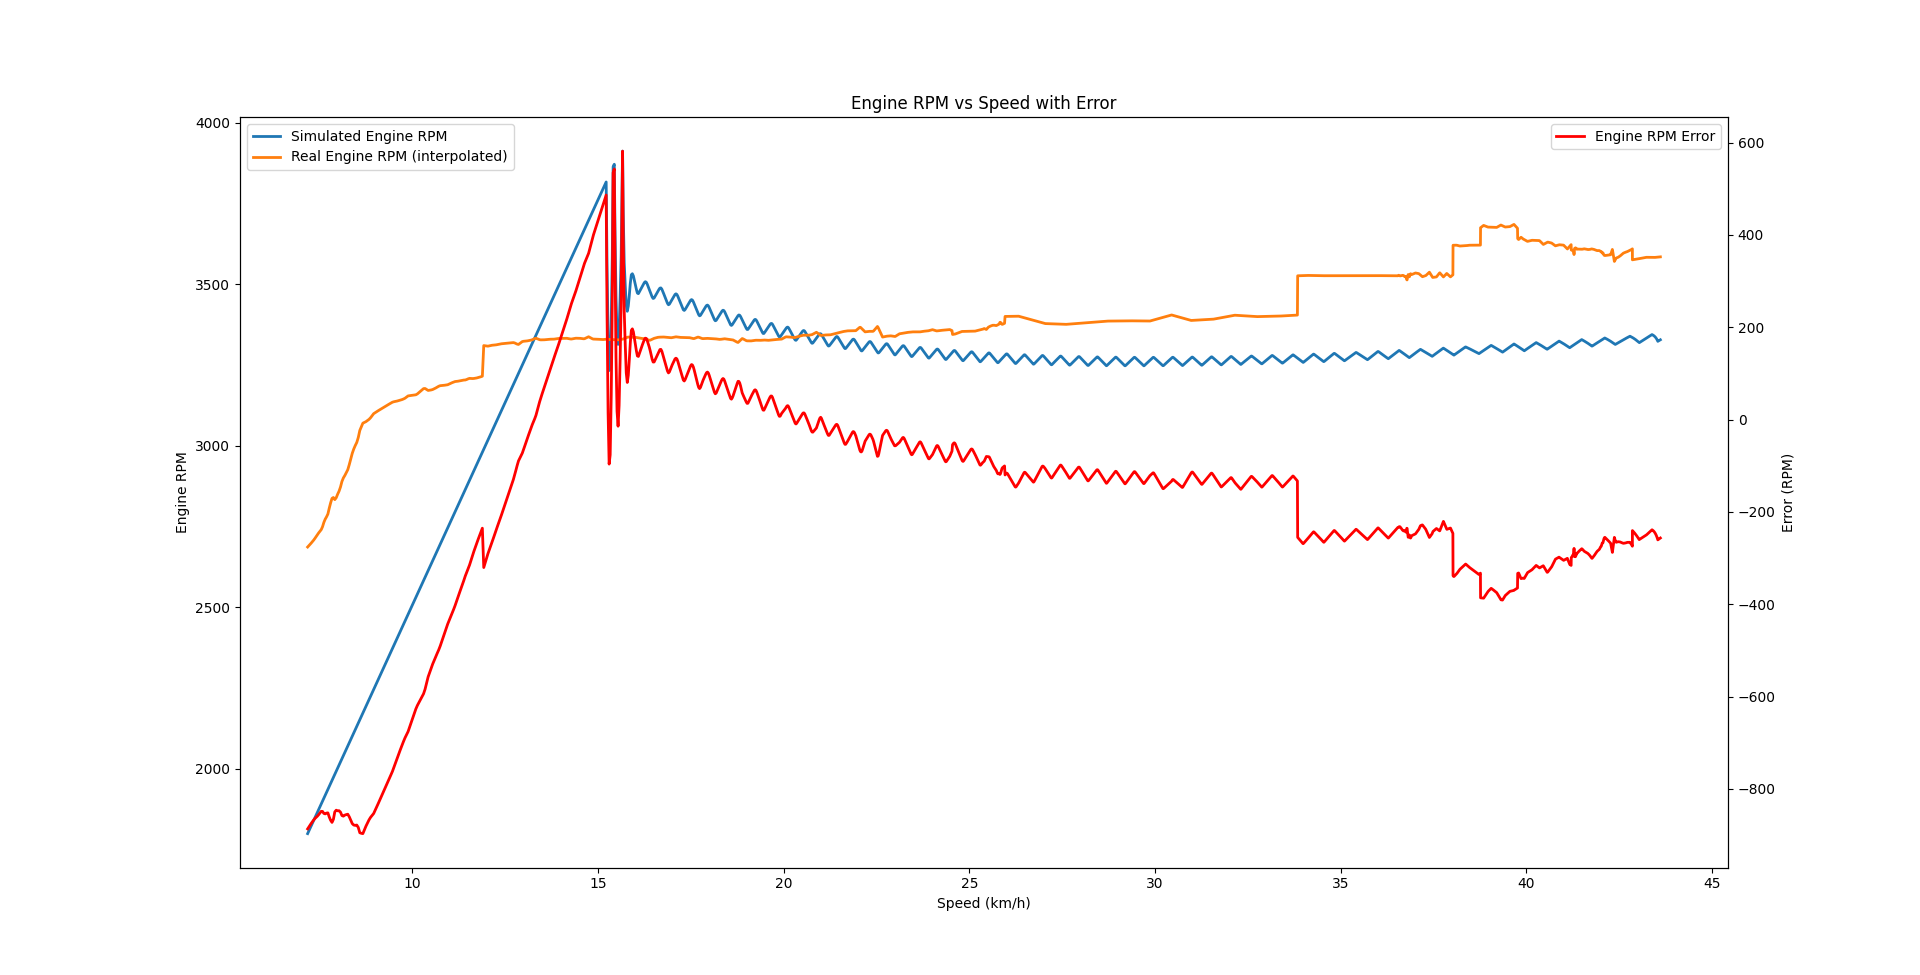
\includegraphics[width=\textwidth]{MSE Graphs/shift_curve_low_ratio.png}
  \caption{Second dataset at a different tune, showing the shift curve and experimental data.}
  \label{Fig_Shift_Low_Ratio} 
  \end{center}
\end{figure}

\textbf{Overview of Shift Curves:}\\
Each figure presents engine RPM vs.\ speed for a distinct CVT tune, where one tune shifts at a higher RPM than the other. This behavior aligns with expectations: reducing weight in the CVT assembly leads to higher shift RPMs. Despite some overall inaccuracy indicated by the consistent error, the relative change in the system (i.e., higher or lower shift points) appears correct.

\textbf{General Observations:}
\begin{itemize}
    \item \textbf{Shifting Direction:} The curves shift as intended, with the tune having less weight achieving higher RPM before shifting.
    \item \textbf{Consistent Errors:} The error trends suggest a systematic mismatch between the model and reality, but the tuning differences themselves manifest correctly.
    \item \textbf{Limited Data Collection:} We do not see the maximum shift range because the test track is too short, preventing the vehicle from reaching top speed and thus limiting the observable shift.
\end{itemize}

\textbf{Comparison of Real vs.\ Simulated Data:}
\begin{itemize}
    \item \textbf{Flat Shift Region:} Both simulated and real data exhibit a generally flat shift region, indicating that the fundamental mechanism of ratio change is captured.
    \item \textbf{Low Ratio Presence:} Each tune shows a low ratio phase, though the exact values differ. This discrepancy may arise from factors such as incorrect geometric assumptions or machining tolerances in the CVT components.
\end{itemize}

\textbf{Potential Sources of Error:}
\begin{itemize}
    \item \textbf{Low Ratio Variation:} Deviations in the low ratio can stem from inaccuracies in modeled geometry, part precision, or an unaccounted slip factor in the real CVT.
    \item \textbf{Shift Curve Nuances:} Subtle variations in the ramps or spring characteristics may lead to unexpected curvature in the shift profile. In the actual CVT system, springs can bind or behave non-linearly under compression, introducing forces not accounted for in the simulation.
    \item \textbf{Slipping Effects:} Occasional slipping in the CVT can alter the effective gear ratio. If slipping occurs, the low ratio appears different because the loss of traction changes the power transfer dynamics, contributing further to the discrepancy between simulated and real data.
\end{itemize}

\section{Trace to Requirements or Modules}

Below are traces of the functional requirements from the \href{https://github.com/gr812b/CVT-Simulator/blob/develop/docs/SRS/SRS.pdf}{SRS}
and the modules from the \href{https://github.com/gr812b/CVT-Simulator/blob/develop/docs/Design/SoftArchitecture/MG.pdf}{MG} to the tests.

\begin{table}[h!]
  \centering
  \begin{tabular}{|c|c|c|c|}
  \hline
    & Position & Velocity & Shift \\
  \hline
  R:MM         &X&X&X \\ \hline
  R:AV         &X&X&X \\ \hline
  R:VV         & &X&  \\ \hline
  R:DV         &X& &  \\ \hline
  R:PCF        & & &X \\ \hline
  R:SCF        & & &X \\ \hline
  R:SA         & & &X \\ \hline
  R:BA         & & &X \\ \hline
  R:ENG        & & &X \\ \hline
  R:TP         & & &  \\ \hline
  R:UA         & & &  \\ \hline
  R:UI         & & &  \\ \hline
  R:DG         & & &  \\ \hline
  R:ER         & & &  \\ \hline
  R:AA         & & &  \\ \hline
  R:WM         & & &  \\ \hline
  \end{tabular}
  \caption{Traceability Matrix Showing the Connections Between Tests and Functional Requirements}
  \label{Table:trace_requirements}
  \end{table}

  \begin{table}[h!]
    \centering
    \begin{tabular}{|c|c|c|c|}
    \hline
      & Position & Velocity & Shift \\
    \hline
    M1        & & &  \\ \hline
    M2        & & &  \\ \hline
    M3        & & &X \\ \hline
    M4        & & &X \\ \hline
    M5        & & &X \\ \hline
    M6        & & &  \\ \hline
    M7        &X&X&X \\ \hline
    M8        & & &  \\ \hline
    M9        & & &  \\ \hline
    M10       & & &  \\ \hline
    M11       &X&X&X \\ \hline
    M12       & & &  \\ \hline
    M13       & & &  \\ \hline
    M14       & & &  \\ \hline
    M15       & & &  \\ \hline
    M16       & & &  \\ \hline
    M17       & & &X \\ \hline
    M18       & & &X \\ \hline
    \end{tabular}
    \caption{Traceability Matrix Showing the Connections Between Tests and Modules}
    \label{Table:trace_modules}
    \end{table}

\end{document}